En la figura \ref{fig:sin_paralelizacion_datos} se presenta una aplicación que
está corriendo sobre un núcleo aleatorio en un ordenador. En este ejemplo no se tiene
presente la paralelización, $D$ representa los datos sobre los cuales está
trabajando la \textit{Aplicación}.

\begin{figure}[h]
  \centering
  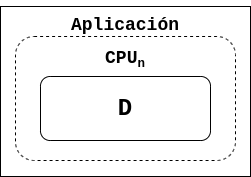
\includegraphics[width=0.3\linewidth]{figuras/procesamiento_paralelo_sin_paralelizacion_datos.png}
  \caption{Aplicación sin paralelización}
  \label{fig:sin_paralelizacion_datos}
\end{figure}
